\documentclass{article}
\usepackage{amsmath}
\usepackage{amssymb}
\usepackage{tikz}
%\usepackage{biblatex}
%\usepackage[style=ieee, sorting=ynt, doi=false,isbn=false,url=false,eprint=false, defernumbers=true]{biblatex}
%\addbibresource{papers.bib}
\usepackage{graphicx}

\title{Codec Classifier}
\date{November 17, 2023}

\newcommand{\Rset}{{\cal R}}

\begin{document}

\maketitle

This paper describes a classifier architecture consisting of an encoder and a decoder.  The word ``codec'' in the name Codec Classifier follows from merging the words en{\it co}der and {\it dec}oder.

\begin{figure}
  \begin{center}
  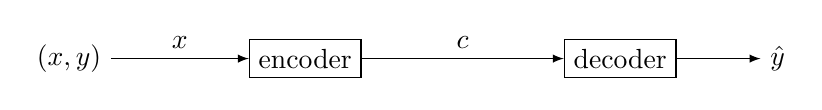
\begin{tikzpicture}[>=latex]
    \node at (-1,0) (x){$(x,y)$};
    \node at (2,0)[draw] (enc){encoder};
    \node at (6,0)[draw] (dec){decoder};
    \node at (8,0) (y){$\hat{y}$};
    \draw[->] (x.east) -- (enc.west) node[above,midway]{$x$};
    \draw[->] (enc.east) -- (dec.west) node[above,midway]{$c$};
    \draw[->] (dec.east) -- (y.west);
  \end{tikzpicture}
\end{center}
\caption{Structure of the codec classifier.}
\label{fig:arch}
\end{figure}

The architecture of the codec classifier is shown in Fig.~\ref{fig:arch}.  An input feature vector $x$ is input to the encoder, which outputs a codeword $c$, which is decoded to a predicted class label $\hat{y}$.  This classifier architecture is reminscent of a communication system.  In communication systems,
\begin{itemize}
  \item the codeword is a perfect representation of the message $x$ with redundancy added to detect and correct errors,
  \item a channel (not shown in Fig.~\ref{fig:arch}) corrupts the bits of the codeword, and
  \item the decoder attempts to recover the message $x$.
\end{itemize}
The decoder's ability to determine $x$ without errors depends on the extent of the channel distortion.

In the classification problem,
\begin{itemize}
\item it is hoped that the codeword $c$ is a perfect representation of the feature vector $x$, but the encoder may be lossy in the sense that $x$ may not be recoverable from $c$,
\item there is no channel, or the channel may be considered to be perfect, i.e. does not induce errors on $c$, and
\item the decoder may be lossy in the sense that even if $x$ is recoverable from $c$, the decoder may not be able to perform that recovery due to the complexity of the recovery problem.
\end{itemize}
In the inferrence step of the classification problem, the goal is to identify the class $y$ associated with an observed $x$.

In communication systems, mutual information is used as a metric to design schemes that make the best use of the channel.  For classification, we adopt the mutual information as a metric to design the encoder and decoder.  We also use the Bayes error as a metric to evaluate different designs.

Consider an encoder consisting of $d$ classification trees having binary codes in the leaves.  A tree with $r$ layers of decision nodes has $2^r$ leaf nodes.  The tree input $x$ selects a leaf node and the leaf's $r$-bit code is output.  Concatenating the results of $d$ trees together yields a $dr$-bit codeword $c$.   A tree with $r=1$ is called a stump.  A stump outputs one bit.  The parameters of a tree are the feature indexes $f_i$, thresholds $t_i$, and $r$-bit codes assigned to the leaves.  The tree output results from a sequence of decisions $x_{f_i} \leq t_i$ that are controlled by the elements of the input feature vector $x$.  When $x_{f_i} \leq t_i$ is true, the decision tree is descended to the left child node and descends to the right child node otherwise.  The classifier design problem chooses the parameters to maximize mutual information or minimize Bayes error.  Under certain conditions, the AdaBoost algorithm is known to minimize the Bayes error.  Therefore, this work builds the encoder with $d$ trees using AdaBoost.

In a multi-class classification problem the AdaBoost classifier may be designed in multiple ways.  Here we offer two possibilities.  First, the standard multi-class AdaBoost approach may be used.  Another possibility is to randomly divide the classes into two sets and train a binary classifier on the sets using the weights from the boosting process.

Suppose the encoder is constructed from $d$ stumps.  Each stump splits feature space into two halfspaces in which the separating hyperplane is aligned with one of the axes.  A stump outputs a 0 for all inputs $x$ in one halfspace and a 1 for all points in the other halfspace.  Put another way, the inverse images of 0 and 1 are axis-aligned halfspaces.

The inverse image of a codeword $c$ is a hyperrectangular set constructed by intersecting one halfspace region from each tree depending on whether the codeword bit is a 0 or a 1.  Codewords and hyperrectangles are in one-to-one correspondence so that we may think of the list of hyperrectangles being indexed by binary codewords.  The hyperrectangles partition feature space into disjoint sets that cover the space.  There are $2^d$ hyperrectangles.  Some of these rectangles may be empty sets.  In that case, the correponding codewords would never be observed at the output of the encoder.

An example classification problem may help to set ideas about the magnitudes of the values involved.  The MNIST dataset consists of $28 \times 28$ 8-bit grayscale images of handwritten digits.  Each image consists of $28^2=784$ pixels.  Each pixel may take on $2^8=256$ values.  Thus there are $(2^8)^{784} = 2^{6272} \approx 10^{1888}$ different images possible.  Suppose we use AdaBoost to build an encoder of $d=1000$ stumps.  There are $2^{1000} \approx 10^{301}$ possible codewords.  Thus, in this case there are not enough codewords to assign a unique codeword to each image.  However, we suppose that feature space may be partitioned into $2^{1000}$ hyperrectangular regions such that a unique codeword can be assigned to each region.  If the regions are pure in the sense that they contain data points from only one class, then the codeword $c$ uniquely represents the class and the decoder design problem is to perform that decoding error free.

An optimal decoder would be an array of $2^d$ elements, i.e. a look-up-table, one element for every hyperrectangle, addressable by the $d$-bit codeword $c$, and storing the class lable $\hat{y}$ for points falling into the corresponding hyperrectangle.  Unfortunately, storing this array exceeds the memory capacity of any conceivable computer for the MNIST dataset and for most other interesting classification problems.  Therefore, we are forced to consider suboptimal approximations of the big look-up-table.

Consider a computer with memory capacity that can store a $2^m$-element array addressed by an $m$-bit word.  This array approximates the $2^d$-element array by sampling $m$ bits out of the $d$ bit codeword $c$.  The particular $m$ bits used may be found by searching over the ${d \choose m}$ combinations of $m$ bits.  However, in interesting classification problems ${d \choose m}$ is so large a number that this search is computationally infeasible.  What is needed is a decoder that approximates the optimal decoder using limited memory and limited computational resources.  We note that heuristic searches such as simulated anealing may find good $m$-bit subcodewords, but we do not pursue this approach further here.

Let $a_{m}$ be an array with $2^m$ elements.  If $w$ is a $m$-bit word, $a_m[w]$ is the corresponding element from array $a_m$.  Let $\sigma_m$ be a selection operator such that $w=\sigma_m(c)$ is an $m$-bit word whos values are selected from codeword $c$.  Composing $\sigma_m$ and $a_m$ gives a definition for a {\it selective array} $a_m[\sigma_m(c)]$, which accesses elements in a small array $a_m$ using select bits $\sigma_m(c)$ from the big codeword $c$.

A tractable, storable approximation to the big look-up-table consists of multiple layers of selective arrays.  Each layer consists of a parallel collection of $d^l$ distinct selective arrays
arrays in which each array is addressed by an $m^l$-bit word.  Each array outputs one bit.  These bits are collected into a $d^l$-bit codeword, which is taken as the input to the selective arrays in the next layer for $l=1, 2, \cdots, L$.  The array in the last layer stores class labels.  The complexity of each layer is determined by the pair $(d^l,m^l)$.  An example network of selective arrays is $(100,5), (50,5), (20,5), (1,20)$.  In this case the last layer has one large array.  The memory requirement is $100 \times 2^5 + 50 \times 2^5 + 20 \times 2^5 + 2^{20} = 5440 + 2^{20} = 1,054,016$ elements.  Most of the memory is for the final array.

The parameters in the proposed decoder are the indexes in the selection operators and the 0/1 bit values stored in the arrays.  We propose a strategy like bagging for finding the selection indexes in $\sigma_m$.  A set of 10 indexes from the input codeword are chosen at random.  Then a ${10 \choose 5}$-way brute force sesarch is performed to select the best 5 from the 10 randomly chosen.  For each five indexes tested, the binary values stored in the array elements are searched at random.  For five bits, there are 32 array elements and $2^{32}$ different combinations possible.  That is too many to exhaustively search.  If instead of 5 bits selected, there were 4, then there would be 16 elements in the array and $2^{16}=65,536$ possible bit configurations.  That might be a small enough number to try all possibilities.  The objective to be maximized during the search is mutual information until the last stage when class labels are output and Bayes error can be minimized, maximizing mutual information between the codeword at the layer output and the input $x$ can be used for optimization.

We note that not all bit patterns need to be tested in the arrays.  For example, an all-zero or all-one array does not help with classification.  Similarly, an array in which the output bit is controlled by one or a few bits in the input word could produce the same output using fewer input bits.  Taking this into consideration only reduces the total number of possiblities by about half, which is not a significant savings.

We propose a greedy approach to optimizing the selective arrays following concepts from building classification trees.  Randomly select a set of bits from the word at the layer input.  Due to the binary nature of the bits, only one splitting point need be considered, $t=0.5$.  Evaluating whether this is a good variable for splitting, calculate the mutual information instead of entropy or Gini index as are commonly used in classification trees.  The mutual information may be evaluated between the class labels $y$ or the data vectors $x$ themselves and the output bits from the split in question.  After selecting a variable for ``splitting'', the dataset is divided and more splits are considered on the next level.  These trees may be grown either sequentially or in parallel.  Note that this architecture leads to a deep network of trees which we call a deep tree network (DTN).

\section{Metrics: Bayes Error}

This section explores Bayes error as a metric for designing coders or decoders for classification.  The Bayes error is the lowest error that can be achieved by any classifier for a classification problem.  Let $f_i = f(x|i)$ be the conditional probability of observing $x$ given that the class is $i$, and let $p_i$ be the priori probability of class $i$.  Then $p_if_i$ is proportional to the posterior probability of $i$ given $x$.  An optimal classifier uses the rule $\hat{i} = \arg\max_i p_i f_i$.  The error associated with this classifer (i.e. the Bayes error) may be computed as
\begin{gather*}
{\cal E} = \int_{p_1 f_1 \leq p_2 f_2} p_1 f_1 dx + \int_{p_1 f_1 \geq p_2 f_2} p_2 f_2 dx. 
\end{gather*}
To simplify the notation, let's define the following shorthand
\begin{gather*}
\int_\leq = \int_{p_1 f_1 \leq p_2 f_2} dx, \qquad \int_\geq = \int_{p_1 f_1 \geq p_2 f_2} dx
\end{gather*}
so that the Bayes error may be written as
\begin{gather*}
{\cal E} = \int_\leq p_1 f_1 + \int_\geq p_2 f_2.
\end{gather*}
Then
\begin{align*}
{\cal E} &= \int_\leq p_1 f_1 + \int_\geq p_2 f_2 \\
&= \frac{1}{2} \left( \int_\leq p_1 f_1 + \int_\geq p_2 f_2 + \int_\leq p_1 f_1 + \int_\geq p_2 f_2 \right) \\
&= \frac{1}{2} \left( \int_\leq p_1 f_1 + \int_\geq p_1 f_1 + \int_\geq p_2 f_2 + \int_\leq p_2f_2 + \int_\leq (p_1 f_1 - p_2f_2) + \int_\geq (- p_1 f_1 + p_2 f_2) \right) \\
&= \frac{1}{2} \left( \int (p_1 f_1 + p_2 f_2) + \int_\leq (p_1 f_1 - p_2f_2) + \int_\geq (- p_1 f_1 + p_2 f_2) \right) \\
&= \frac{1}{2} \left( \int (p_1 f_1 + p_2 f_2) - |p_1 f_1 - p_2f_2| \right) \\
&= \int p_2 f_2 - \int p_2 f_2 + \frac{1}{2} \left( \int (p_1 f_1 + p_2 f_2) - |p_1 f_1 - p_2f_2| \right) \\
&= p_2 + \frac{1}{2} \left( \int (p_1 f_1 - p_2 f_2) - |p_1 f_1 - p_2f_2| \right) \\
&= \min(p_1,p_2) + \max(p_2-p_1,0) - \frac{1}{2} \left( \int f_2 \left[\left(p_2 - p_1 \frac{f_1}{f_2}\right) + \left|p_2 - p_1\frac{f_1}{f_2}\right| \right]\right) \\
&= \min(p_1,p_2) - \int f_2t\left(\frac{f_1}{f_2}\right), \\
&= \min(p_1,p_2) - E_{f_2} t\left(\frac{f_1(X)}{f_2(X)}\right) \\
t(x) &= \frac{1}{2} \left[ (p_2-p_1 x) + |p_2 - p_1 x|\right] - \max(p_2-p_1,0) \\
&= \max(p_2-p_1x,0) - \max(p_2-p_1,0).
\end{align*}

A $f$-divergence between two density functions $f_1$ and $f_2$ is defined as
\begin{gather*}
D_g(f_1 || f_2) = \int f_2(x) g\left(\frac{f_1(x)}{f_2(x)} \right) dx = E_{f_2} \left[g\left(\frac{f_1(X)}{f_2(X)}\right)\right],
\end{gather*}
where $g$ is a smooth and convex function such that $g(1) = 0$.  The KL-divergence, Hellinger distance, and total variation distance are special cases when $g(x) = x \log(x), (1-\sqrt{x})^2, \frac{1}{2} |x-1|$, respectively.  Observe that $t$ satisfies the properties required in the definition of $f$-divergence: $t(1) = 0$ and $t(x)$ is a convex function.  Thus, the expression for the Bayes error above shows it able to be written as an f-divergence between conditional densities $f_1$ and $f_2$.

\subsection{Using Bayes Error with Data}

When observations of $x$ are available under $f_1$ and $f_2$, the ensemble average is replaced by a sample average
\begin{gather*}
\hat{{\cal E}}(X_1,X_2) = \min(\hat{p}_1, \hat{p}_2) - \frac{1}{N_2} \sum_{i=1}^{N_2} \tilde{t}\left(\hat{U}_i\right),
\end{gather*}
where $\tilde(t)(x) = \max(t(x),t(C_L/C_U))$, $0 < C_L \leq f_1(x), f_2(x) \leq C_U$, and $\hat{p}_1,\hat{p}_2$ are emperical estimates (relative frequencies) of the class labels in the training set.  $\hat{U}_i$ is an estimate of the density ratio at point $x_i$ with class label 2, which is computed based on the data points falling into an $\epsilon$-ball about $x_i$, and $N_2$ is the number of class 2 points.

A symmetric version of Bayes error is
\begin{gather*}
{\cal E}_\epsilon = \frac{N_2}{N} \hat{{\cal E}}(X_1,X_2) + \frac{N_1}{N}\hat{{\cal E}}(X_2,X_1) = \min(\hat{p}_1, \hat{p}_2) - \frac{1}{N} \sum_{i=1}^{N} \tilde{t}\left(\hat{U}_i^\epsilon\right),
\end{gather*}
where $\hat{U}_i^\epsilon$ is the density ratio estimate using a $\epsilon$-ball about the point $x_i$ (see Noshad's thesis for the definition).  Estimates for various values of $\epsilon$ may be combined to improve convergence behavior.  See Noshad's thesis for more information.
Noshad's thesis also presents a multi-class version of the Bayes error estimator.

\section{Mutual Information}

\subsection{Nearest Neighbor Ratio (NNR)}

The NNR provides estimates of divergence (either Renyi divergence or $f$-divergence).  The NNR estimate of mutual information is obtained by constructing a second dataset in which the class labels are randomly permuted leading to independence between the features and the labels.  These two datasets are passed into a divergence measure
\begin{gather*}
\hat{I}(X,Y) = \hat{D}((X,PY) || (X,Y)).
\end{gather*}
See chapter 2 in Noshad's thesis for more information on this approach.  A randomized and ensemble version of NNR are also presented with improved performance.  I tend to think that the basic NNR would be sufficient for training/learning the selective arrays by greedy tree building methods.  In this case, we are trying to maximize the mutual information between the input features or their class labels and the binary codes produced in the layers of the trees being built to approximate the selective arrays.  In building a tree that approximates a selective array, splits on various input variables (bits from the codeword produced in the previous layer) are considered.  To evaluate the fitness of any split, pass the training data through the classifier up to the previous layer.  Pass the codeword for each input through the split in question.  This gives a base dataset.  Construct a second dataset in which the class lables are randomly permuted.  Use these two datasets to evaluate a the NNR estimate of mutual information.  One question is whether to use a different random permutation every time or to reuse the same random permutation multiple times when comparing splits on different input variables.  I tend to think that the same permutation should be used when comparing the splits on different input variables because we don't want the randomness in the permutation to bias the variable selection process.  Perhaps several permtuations should be used and the results averaged together to reduce bias.

Maybe this fancy mutual information estimation is unnecessary because our data are discrete and we can simply use histogram estiamtes.  The class labels are few in number and the bits in the binary codes are binary valued.  With a large dataset, the histogram estimates might work very well.

\section{Methodology}

The proposed learning process consists of two steps: (1) learning the encoder that exhaustively segments the input feature space, and (2) learning a decoder that exhaustively labels each region in the segmentation.

\subsection{Encoder: Exhaustive Segmentation}

The first step keeps adding trees or stumps until the feature space is segmented into pure regions or until a desired error rate is achieved.  Pure regions would give zero error on the training set.  The overall classifier will achieve no better error rate than what is enabled by the segmentation.  The tradeoff is that achieving pure regions may require dramatically more regions than achieving a non-zero error rate.  Thus error rate may be used to control the size of the encoder layer.

\subsection{Decoder: Exhaustive Labeling}

An ideal decoder will assign a label to each region created by the encoder.  Because this is usually not possible, a practical decoder, which is subject to memory constraints for storage and to compoutational constraints during learning, is suboptimal.  Finding the optimal is a constrained optimization problem.  Among many options available, we explore the use of bagged or boosted trees to perform a greedy search.

\section{Encoder Training}

In a $k$-class learning problem, two approaches for encoder learning will be explored.  The goal with both approaches is to exhaustively segments (zero error on the training set) or approximately segments (training set error below a predetermined allowable error rate).

\subsection{Approach 1: $k$-class boosting}

The first approach employs the standard multi-class AdaBoost algorithm which augments the objective function with a $k$-dependent term.  The resulting trees contain $k$-element probability vectors in the leaves.  These vectors express the relative frequency of points from the training set that fall into the region corresponding to the leaf.  Pure regions yield one-hot vectors.

\subsection{Approach 2: Randomized Binary Boosting}

The second approach employs a modification to the standard algorithm for binary AdaBoost for learning.  The modification involves two steps.  On each iteration, before the next tree is built, the dataset is divided into two classes rather than $k$-classes.  This is done by a process we call ``splitting the deck''.  As in playing a card game, the class labels are treated as cards, the cards are shuffled to randomize them, and then the deck of cards is randomly split into two sets.  This may be accomplished in code using a random permutation followed by generating a random split point according to some distribution such as a uniform distribution or another distribution such as a binomial distribution that is biased toward splitting the deck in half.  Following this deck-splitting operation, one set of classes is considered the ``0'' class and the other set of classes is considered the ``1'' class.  The next tree is trained to minimize error on this binary segmentation of the dataset.

Why does randomized binary boosting (RBB) properly segment the input feature space?  In simple terms, a classifier that discriminates based on a fine attributes is able to classify based on course attributes.  RBB uses this concept in reverse.  It by learning binary classification on multiple random binary splits of the training data, it learns the finer segmentation.


Let $g$ be a $k$-class classifier $g(x) = i$ if $x \in R_i$ for $i \in I = \{1, 2, \cdots, k\}$, where $R_i$ is the region of the input feature space where the classifier chooses class $i$.  We note that the $R_i$ are disjoint and cover feature space.

Let $h$ be a binary classifier derived from $g$ via a random deck-shuffling operation.  Let $I_a$ and $I_b$ be disjoint index sets corresponding to class $a$ and class $b$ respectively, $I=I_a \cup I_b$.  Let $R_a = \cup_{i \in I_a} R_i$ and $R_b = \cup_{i \in I_b} R_i$ be a disjoint binary partition of the input feature space.  Then $h(x) = a$ if $x \in R_a$ and $h(x) = b$ otherwise.

The error rate of $h$ is
\begin{align*}
{\cal E}_h &= \int_{R_b} p_a f(x|a) dx + \int_{R_a} p_b f(x|b) dx \\
&= \sum_{j \in I_b} \int_{R_j} p_a f(x|a) dx + \sum_{j\in I_a} \int_{R_j} p_b f(x|b) dx \\
&= \sum_{i \in I_a} \sum_{j \in I_b} \int_{R_j} p_i f(x|i) dx + \sum_{i \in I_b} \sum_{j \in I_a} \int_{R_j} p_b f(x|b) dx.
\end{align*}

The error rate of $g$ is
\begin{align*}
{\cal E}_g &= \sum_{i \in I} \sum_{j\neq i} \int_{R_j} p_i f(x|i) dx \\
&= \sum_{i \in I_a} \sum_{j \neq i} \int_{R_j} p_i f(x|i) dx + \sum_{i \in I_b} \sum_{j \neq i} \int_{R_j} p_i f(x|i) dx\\
&= \sum_{i \in I_a} \sum_{j \in I_b} \int_{R_j} p_i f(x|i) dx + \sum_{i \in I_a} \sum_{j \in I_a, j\neq i} \int_{R_j} p_i f(x|i) dx \\
&+ \sum_{i \in I_b} \sum_{j \in I_a} \int_{R_j} p_i f(x|i) dx + \sum_{i \in I_b} \sum_{j \in I_b, j\neq i} \int_{R_j} p_i f(x|i) dx\\
&= {\cal E}_h + {\cal E}_{g,a} + {\cal E}_{g,b}, \\
{\cal E}_{g,a} &= \sum_{i \in I_a} \sum_{j \in I_a, j\neq i} \int_{R_j} p_i f(x|i) dx,\\
{\cal E}_{g,b} &= \sum_{i \in I_b} \sum_{j \in I_b, j\neq i} \int_{R_j} p_i f(x|i) dx,
\end{align*}
where ${\cal E}_{g,a}$ and ${\cal E}_{g,b}$ are the error rates for the $k$-class classifier for particular kinds of errors.  ${\cal E}_{g,a}$ counts errors to classes in the set $I_a$ when $i \in I_a$, and the same for ${\cal E}_{g,b}$.  

Thus we see that the $k$-class error rate is equal to the binary error rate plus the sum of the within class error rates ${\cal E}_{g,a}$ and ${\cal E}_{g,b}$.  However, we note that the error rates derived above are random variables that depend on the distribution of the deck-shuffling operation.  The proposed training process effectively minimizes the binary error rate over multiple draws of deck-shuffling.  Each draw randomizes the membership of classes $a$ and $b$ in the binary problem.  Minimizing the binary error over random draws will minimize the within class error rates.  Thus the $k$-class error rate is minimized in turn. (Need to prove this claim rigorously.)

\section{Training the Decoder}
We have described a classifier architecture consisting of an encoder that splits up feature space into many segments and outputs a codeword for all feature vectors falling into the corresponding region.  The decoder converts the codeword into a class label.  Training the decoder can be done by several means.

\subsection{Single Decision Tree}
A single large decision tree may be grown.  Evaluating splits at each decision node is easy because of the binary nature of the input.  There is only one split to consider for each input feature index.  This means that we could probably try splitting on all of the possible input variables at each decision node.  This grows exponentially with the depth of the tree because each layer doubles the number of decision nodes.  Keep growing the tree until leaf nodes are pure or until some probability of error is reached.  The large tree acts like a look-up table.  How is this different from simply growing one large tree on the original input data?

\subsection{Boosting Trees}
Boosting a layer of small trees may be used for the decoder.  If we sample at random the bits of the input codeword, then this method uses trees like small selective arrays.  Boost a layer of these.  Because the tree inputs are binary, the expensive threshold sweep is not needed.  There is only one possible split point that needs to be evaluated at each decision node.  This means that more indexes can be explored at each decision node.  The trees output binary codes until the last layer where an actual selective array is used.  This array holds the class indexes.

\subsection{Boost Selective Arrays}
A collection of selective arrays could be trained using boosting.  The array size is fixed at say 1kB.  Array elements are probability vectors for the class labels.  Selecting several bits from the input codeword groups together regions in the input space.  This is done multiple times at random and the best resulting array is kept as the weak learner.  This process is boosted using the AdaBoost algorithm that increases weights on mis-classified values.

\section{Is the the coder-decoder architecture a good idea?}
Before taking up the main question, we need to introduce some terminology.  The codec classifier uses binary codes in the leaf nodes of the trees in the encoder.  In general for classification and regression problems, there is no need to require leaf values to be crisp binary values.  Underlying this whole research theme is the is the idea of the encoder producing hard quantized outputs.  Going from feature vectors (raw inputs) to hard quantized values in a single stage may be too abrupt of a transition and may be asking too much of that first stage.  It may be wise to soften the transition through several stages of processing with soft values being passed between the stages.  However, to move the discussion forward, we refer to trees and stumps with binary values in their leaf nodes as bees and bumps instead of trees and stumps.

The main question up for debate about the coder-decoder classifier architecture is whether there is any value beyond what the boosted classifier can already deliver.  Boosting bees/bumps in the first layer produces a classifier
\begin{gather*}
H(x) = \text{sgn}\left( \sum_{i=1}^T \alpha_i h_i(x)\right)
\end{gather*}
that assigns a value to every region in the input feature space.  That partitioning of feature space and the values assigned to each region may be explored using my region adjacency graph framework.  The main question is whether the decoder in the codec-classifier, which has the freedom to make independent assignments to those regions, has any performance improvement to offer beyond what the the boosted classifier $H(x)$ already offers.  It is true that the forward additive modeling of AdaBoost is tightly constrained by the algorithm, but that tight control may be exactly the right thing to do to approach the Bayes error.  The constraints are not necessarily a bad thing.  Our main question is then what does the codec-classifier architecture offer.  It's encoder breaks apart the weak learners $h_i(x)$ and doesn't formally use $H(x)$ at all.  Instead, it uses each bee/bump $h_i(x)$ to produce bit(s) in the codeword.  The codeword indexes a region that gets a constant class assignment $\hat{y}$.

Perhaps the best way to analyze this situation is to start by using the ideal decoder which is an array of $2^d$ elements that stores the class label for each region.  Many codewords are associated with empty regions and these array elements then need not be filled.  Does this ideal decoder offer any advantage over AdaBoost?  The ideal decoder must be a superset of the AdaBoost assignment.  So perhaps our analysis should be of AdaBoost itself.  Can we find a situation in which you could do better than AdaBoost with arbitrary region assignments.  To put this another way, the codec-classifier is the most general form of classifier.  It can make arbitrary class assignments to each region.  The AdaBoost classifier is constrained by the additive form $H(x)$ above.  Can we show that this form creates constraints not imposed by the ideal decoder?  Maybe the argument would go like this.

(1) Set the stage by showing that the classifier with $T$ trees splits feature space up into a total of $N$ regions, where
\begin{gather*}
N = \Pi_{i=1}^d (t_i + 1), \qquad \sum_{i=1}^T t_i = T.
\end{gather*}
Here $T$ is the number of trees, $t_i$ is the number of splits in the $i^\text{th}$ dimension and for stumps there is one dimension per tree.  As the number of classifiers grows, the number of regions grows very fast unless the splits all fall in one dimension.  That is unlikely.  So we conclude that we have many times more rectangular regions than we have trees.

(2) The tree combination in $H(x)$ is constrained in the number of values it can take on.  If we started to make assignments of arbitrary values in each region, we loose one degree of freedom for each region arbitrarily assigned.  We run out of degrees of freedom after assigning $T$ alpha values $\alpha_i$.  So if we have more regions than stumps, it's game over for the stumps and the ideal decoder offers more flexibility.

I think we could prove this even in one dimension.  Suppose you have two stumps with a one dimensional input space.  Two stumps gives two thresholds and three regions.  But you have only two alpha-parameters to set the values in three regions.  This is not quite right because it does not take into account that each tree has two leaf values that may be assigned arbitrarily.  Need to appeal to the region adjacency graph theory to study the true flexibility of a forest with additive output.  By setting up a system of equations, in which the coefficient vector are the variables, the right hand side is arbitrary, and the coefficient matrix structure is determined by the region adjacency graphs of the trees and their graph products.  Only then will we see what the real structure of this problem is.

Here's a proof in low dimensions giving an example that doesn't work.  In two dimensions have two stumps in both dimensions.  This gives nine regions but the four trees have only eight leaf values to assign.  You can write down a matrix equation with a full column rank $9 \times 8$ matrix, but there is a configuration of class assignments to regions that the forest classifier cannot achieve using the additive model $H(x)$.  This proves that the decoder has more flexibility that the forest classifier.

\section{Related Work}

\subsection{Hashing}

Zhang {\em et al} \cite{fast_knn} describe a method for fast approximate construction of a $k$-nearest neighbor ($k$nn) graph.  They divide a dataset into groups and construct a full $k$nn graph in each group.  The complexity of their method scales with group size.  Division of data into groups is done using hashing in a way that preserves pairwise similarities, i.e. similar items fall into the same group.  This is called locally sensitive hashing (LSH).  In general, a hash has the form
\begin{gather*}
h(x) = [ h_1(x), h_2(x), \cdots, h_m(x) ],
\end{gather*}
where $h_i(x) \in \mathbb{Z}$ (integers).  The specific hash mentioned in the papaer is
\begin{gather*}
h_i(x) = \text{sgn}(w_i^T x + b_i) \in \{-1, +1\},
\end{gather*}
where $w_i$ and $b_i$ are parameters to be learned by an unspecified method.  A datapoint $x$ is placed in a "bucket" by applying the hash map $h(x)$ and then using the $m$-digit $\pm 1$ code as the bucket index.  LSH keeps similar points together using a set of sliced (affine) projections.

The fast $k$nn method uses a binary $\{0,1\}^m$ hash code $y = h(x)$ and uses random projection $w$, $p = w^T y$.  To keep similar points together in groups, the $p$ values are sorted and then blocked into groups of the desired size.  Fully $k$nn graphs are constructed from these groups followed by one stage of neighbor-of-neighbor search.  The whole process is repeated several times using different random projections of the hash codes, and the accuracy of the method is a very good approximation to the full $k$nn graph.

This work is interesting and related for several reasons.
\begin{enumerate}
\item Like this work, we propose to use binary codes.  The binary codes in our method may be thought of as a hash.
\item This method uses learned projections $h_i(x) = \text{sgn}(w_i^T x + b_i)$ to build the has.  Our method uses AdaBoost to construct axis-aligned projections $h_i(x) = \text{sgn}(e_i^T x - t_i) \in \{0,1\}$ which is equivalent to the logical condition in a decision node $x_i \leq t_i$ in a decision tree.  The authors do not say how the $w_i$ and $b_i$ are learned in their method.  We follow the principled approach of AdaBoost which has the advantageous claim that it's error approaches the Bayes error (i.e. the best that a classifier can do).
\end{enumerate}

\subsection{Binary and $k$-Class Problems}

Talk in this section about how we propose to handle the $k$-class case either by using multi-class AdaBoost or by using a binary partitioning of the data at each step.  The binary partitioning can be done in multiple ways.  Here we can refer to Singer's one-versus-all splitting or we can follow a random uniform, half-and-half, or $k~$binomial or Poisson splitting.

It may also be a good idea to cover the strong weak learner verses weak weak learner concept here too.

Ji Zhu, Hui Zhou, Saharon Rosset and Trevor Hastie, Multi-class Adaboost. A multi-class generalization of the Adaboost algorithm, based on a generalization of the exponential loss.
Finally published in 2009 in Statistics and Its Interface Volume 2 (2009) 349-360.

This paper discusses many of the early methods at extending AdaBoost to the multi-class case and points out that what they did is basically convert the $k$-class problem into binary problems.  To contrast this with our work, we are not building the encoder/hasher to be a $k$-class classifier or a binary classifier.  We are building the encoder/hasher to segment feature space only and to construct a codeword/hash for each region of feature space.  The decoder assigns labels to the regions.  Therefore, our method for random binary splitting of the classes at each stage of AdaBoost is done for a different reason, and we only need the approach to create good segmentations of feature space.  Whatever method that will do that can be used.  Because we are outputting binary codes, using a $k$-class algorithm does not "fit" our objective.

What does fit our objective is a boosting algorithm that, on every iteration, suffles the classes and "splits the deck" in the sense of dividing the shuffled classes into two sets.  These sets need not be equal in size and we can use a probability distribution to select the splitting.  The question I have is whether the standard weight update in AdaBoost is appropriate to use without modification, or do we need to go back and recompute the weights according to the new binary super-classes?  Recomputing the weights would amount to initializing the weights as uniform and then following only the weight update up to the current stage.  This would give weights that reflect the ability of the current classifier according to the new binary super-classes.  Without recomputing, the weights correspond to how a different classifier (one trained on different binary super-classes) makes errors.  Which one of these approaches is "right" or does it even matter?

\section{Notes on Partitioning}

Most ensemble methods (may be an over-generalization, and may apply to. other techniques as well such as neural networks) for classification perform the space partitioning and function approximation at the same time, by one algorithm, in a single phase.  The codec-classifier separates these two necessary steps into two separate stages.  The encoder performs only the job of space partitioning.  The decoder then assigns class labels to the regions.  How can we partition space in a way that will lead to overall high accuracy without first thinking about classification in that step?  The answer is to design the encoder to maximize the mutual information between the class labels and the codeword at the output of the encoder.  Then the decoder can simply make a hard decision about each region based on the relative frequency of training points falling in those regions, or it can draw at random according to the distribution of points in the region.

Noshad's thesis has chapters on hash-based estimation of divergence and mutual information.  This method relies on a hash that maintains proximities between hash inputs and outputs.  Points that are close together in the input space/feature space should has to the same values.  This is exactly what our encoder does and the codeword output is the hash.  So we can apply the techniques for hash-based mutual information estimation to our problem of training the encoder.  Previously (above in this document), we proposed that AdaBoost be used to train the trees/stumps in the encoder.  However, I have observed that AdaBoost adds trees that do not appear to help the segmentation of the input space but rather help add a DC offset/bias to the additive function value.  Through experimentation I hope to find that mutual information, which does not maintain a function the way that AdaBoost and other methods do, will be more effective at utilizing every tree purely for segmenting the input/feature space in ways that directly help classification.  This separation of responsibilities between encoder and decoder and the adoption of mutual information as a metric to design the encoder appear to be novel.  If we cannot store the ideal decoder and must use an approximation scheme, we can draw upon AdaBoost or mutual information to learn a set of selective arrays or trees to approximate the ideal decoder with low error.

\section{Experiments}

I have just completed some experiments in Matlab.  I started with my AdaBoost code and ripped out the weight calculations and replaced the error metric with hash-based mutual information metric.  After banging my head against a wall using Matlab's dictionary with buggy insert and remove functions that don't work properly, I have found that the mutual information (MI) metric works splendidly well at segmenting space.  Once the segments reach purity, the MI flattens out and is a constant over all further splits.  Splitting can stop at this point and then region assignments can be made in the decoder.  What I had hoped would work, does in fact work.

What I am also seeing is that MI creates these tiny sliver regions to isolate a "0" class point in the midst of a sea of "1" points.  Then the resulting regions become pure.  [Show an example.] Is this behavior that we want?  We can post process and remove sliver regions based on their volume or minimum coordinate width.  Or we could regularize the whole process by stopping splitting once the region purities drop below a threshold or when the MI drops below a threshold.  Remember that the decoder can be a hard decision decoder, storing the index for the class assigned to that region, or it can be a stochastic assignment, storing the relative frequency for that region and then drawing a class label at inference time based on the relative frequency vector for the region.

Aside.  In fact, this may be an entirely different approach to classification altogether.  Instead of learning class labels for regions or probability assignments for a region, if we could come up with a class pdf for each point in feature space, then we could always draw at inference time according to that pdf.  Maybe we could use a Gaussian Process to interpolate across the input space/feature space.  It seems like this sort of inference would be the best for a given set of training data.

\section{New Notes}

Interpretability is an important feature for a classifier.  The codec classifier offers interpretability.  The bits in the codeword together with the feature indexes and thresholds encode all the information about a particular rectangle.  A zero bit $c_i=0$ in a codeword indicates that the rectangle's upper edge in the $f_i$ dimension lies below $t_i$.  A one bit $c_i=1$ in a codeword indicates that the rectangle's lower edge in the $f_i$ dimension lies below $t_i$.  The rectangle's actual upper (lower) edge in dimension $f_i$ is the minimum (maximum) of all the thresholds in that dimension with a zero (one) bit.

In the process of splitting up feature space and due to the global way that stumps and trees divide the space, there may be rectangles that have no training data in them.  Then the question arises at inference time how to classify points that fall into these rectangles.  Here we see an advantage of the codec classifier over other alternatives.  The codec classifier can report no class.  It is essentially saying, "I have never seen any data in this region of feature space so I'm not confident enough to report anything."  In fact, we can go further than this.  In the training process, we can save in the decoder array a frequency count and total count for each rectangular region.  Then when predicting a new point, the codec classifier can report not only a class label, but it can also report a relative frequency and total count for the region.  This gives the user an indication of the confidence.  The codec classifier is essentially saying something like, "In this region I have seen lots and lots of training points and I'm very confident when I say that this is class x."  Or it may be saying, "Well if you want to know what I think, it's class x, but I'm not totally certain, because I've only seen a few instances in this area."  These sorts of statements give way more information than what neural networks can give.  Neural networks slice up feature space and report answers for every input point but say absolutely nothing about (i.e. silent) confidence or nearness to other points.

If pressed to give a response for a point falling in an empty rectangle, the codec classifier could search through adjacent rectangular regions to find a region that is occupied by data points.  The user may take the risk of using the resulting prediction armed with the information about the risk they are taking.  Here's how that search would work.  Essentially we would search through the rectangle adjacency graph.  Information for doing so is in the codeword.  The first step is to search through the dimensions $f_i$ and the thresholds $t_i$ to find the one that is closest to the point (in fact, I recommend making a sorted list).  Then to find the adjacent rectangle, flip the corresponding bit in the codeword and move into the corresponding rectangle.  If that rectangle does not have any data points, then we move through the sorted list to find the next closest rectangle to the original rectangle, or we look at an adjacent rectangle to the adjacent rectangle.  An efficient graph search could be organized using these principles to find a rectangle that does have data points in it.

\section{The "Bug" in AdaBoost}

I'm following the AdaBoost algorithm in Schapire and Freund's book "Boosting: Foundations and Algorithms", MIT Press, 2012, page 5.  This uses 200 data points.  The $+1$ class is 100 zero mean, unit variance Gaussian random variables.  The $-1$ class is 100 unit variance Gaussian random variables with mean drawn uniformly at random from the set $\{ -4, +4\}$.  I ran three iterations of AdaBoost.  The iteration error rates were 0.25, 0.26, and 0.015.  The alpha $\alpha_t$ values were 0.5493, 0.7582, 0.6429.  The figure below shows the unusual behavior of the splitting on the first three splits.  Note that the thresholds are -2.2166, 2.2365, 5.7779.  These are shown as vertical lines in the figure.  It's the unusual behavior of AdaBoost's splitting that is being investigated here.  The first two splits seems reasonable if we are trying to minimize the probability of error, but what is going on with the third split.  It does not seem to be an intelligent split at all.  Why does AdaBoost waste a split way off on the edge?  It does not serve to reduce error.  But actually it does.  This split is required to reset the offset value of the additive overall classifier.  The additive nature of the resulting AdaBoost classifier acts as a constraint and forces AdaBoost to waste many splits simply to reset the vertical bias of the additive function so that when it is thresholded, it will give correct answers.  Let's look into this a bit more.

The additive function is shown after each iteration.  The green line shows the first additive function when there is only one classifier in the split.  The first alpha is 0.5493, so the first split assumes the value -0.5493 on the left and +0.5493 on the right.  The second split point is a good one, but note that the additive classifier now gets a whole bunch of the points on the left wrong when it is thresholded at zero.  This is because the second alpha is 0.7582, greater than the first alpha.  So when the third classifier is considered, it must be chosen to reset the vertical offset of the function.  This is why it is chosen way off to the right.

In conclusion, the additive nature of AdaBoost and other ensemble-type classifiers may be viewed as a constraint that limits the method's ability to make informative splits at each point.  Using mutual information offers an improvement because it does not care about probability of error or additive models.  It simply wants to make informative splits at each step.

\begin{center}
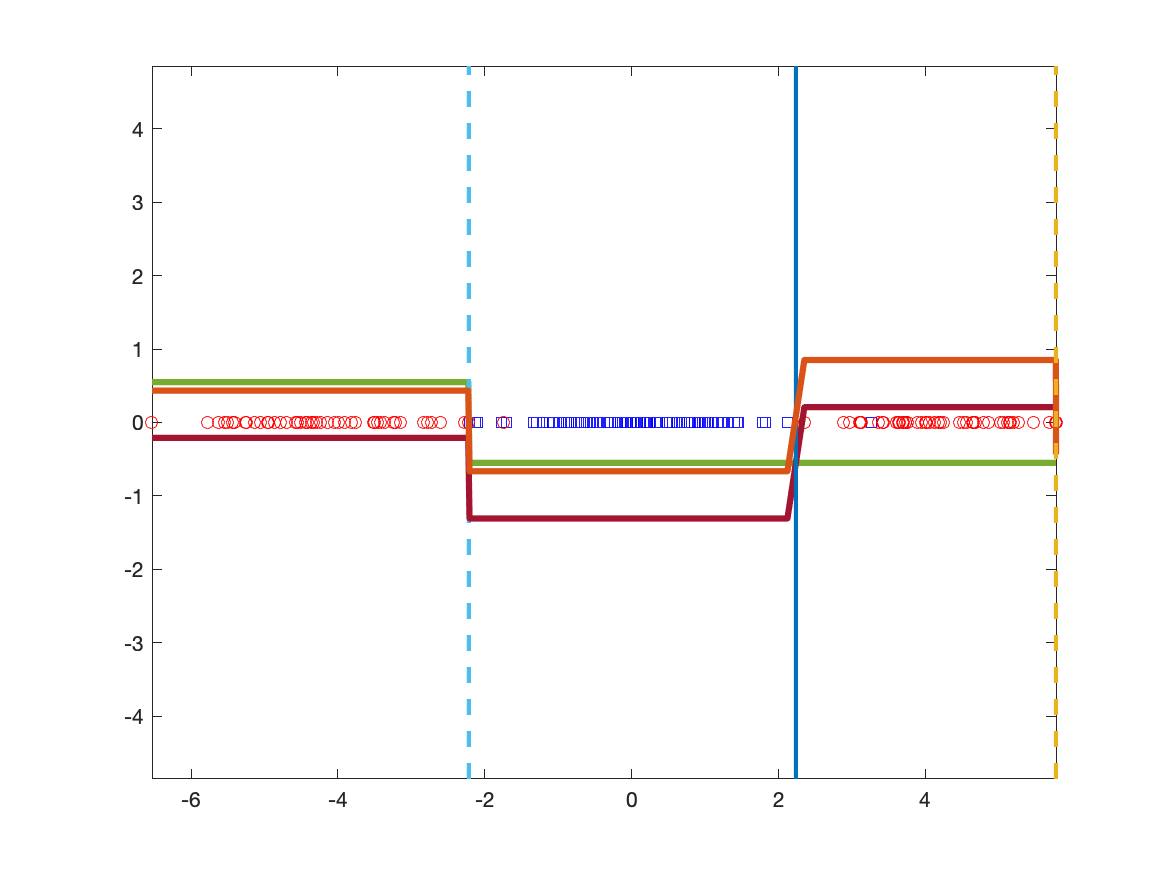
\includegraphics[width=0.8\linewidth]{adaboost_bug.png}
\end{center}

\section{Analytical Behavior of AdaBoost and Mutual Information}

Let $X$ be the set/space of feature vectors.  Usually $X = \mathbb{R}^n$ or a subset thereof.  Let $C: X \rightarrow \{0,1\}^d$ be the encoder mapping, $C(x) = c$, defined by a set of feature index, threshold pairs $(f_i, t_i), \;i=1, 2, \cdots, d$.  The bits in $c$ are defined by the logical condition
\begin{gather*}
c_i = \begin{cases} 0, & x_{f_i} \leq t_i, \\ 1, & x_{f_i} > t_i. \end{cases}
\end{gather*}

Training data are given as pairs $(x_i, y_i)$ for $i=1, 2, \cdots, N$, and we assume that these data are drawn from the distribution $p(x,y) = p(x|y)p(y)$.  The joint probability of a codeword $c(x)$ and $y$ is given by
\begin{align*}
p(c,y) &= p(c|y) p(y) \\
&= \text{Prob}(x_{f_1} \square_{c_1} t_1 \;\; \text{and} \;\; \cdots \;\; \text{and} \;\; x_{f_d} \square_{c_d} t_d | y) p(y) \\
&= p(y) \int_{R_{c}} p(x|y) dx,
\end{align*}
where $\square_{c_i}$ is the appropriate inequality based on the bit $c_i$, $R_{c}$ is the rectangular region determined by the codeword $c$, and $K$ is the number of classes.  We assume that $y \in \{1, 2, \cdots, K\}$.  

The mutual information between $c$ and $y$ is given by
\begin{align*}
I(c,y) &= \sum_c \sum_y p(c,y) \log \frac{p(c,y)}{p(c) p(y)} \\
&= \sum_c \sum_y p(y) p(c|y) \log \frac{p(c|y)}{\sum_g p(c|g) p(g)} \\
&= \sum_c \sum_y p(y) \int_{R_c} p(x|y) dx \log \frac{\int_{R_c} p(x|y) dx}{\sum_g p(g) \int_{R_c} p(x|g)dx}.
\end{align*}
Mutual information encoder design maximizes this expression for MI which is a function of the next feature index $f_{d+1}$ and threshold $t_d$.  This is done in a manner similar to tree/stump design using other metrics.  A scan is performed over all indexes and for each index a threshold is swept over a range of values.

It is interesting to compare the MI expression with the expression for weighted error probability used in AdaBoost.

\section{A Note on the Complexity of the Codec Classifier Decoder}

Once the encoder part of the codec classifier has been trained/learned, the second step is to train the decoder.  The ideal decoder is simply a large array that stores a class label for each rectangle.  When an instance is presented for inference, it is encoded to a codeword and the codeword is used as an index into the large array to look up the class label for that region.  As noted previously, we may look up a data structure that contains other useful information such as the abundance information about training points falling into that rectangle from different classes as well as the total number of points falling into that rectangle.  Because many codewords do not have a non-empty rectangle and many rectangles may not contain training data, it makes more sense to use a map or dictionary data structure to store information for each rectangle.  How large does this dictionary need to be.  Well it's much smaller than $2^d$, where $d$ is the number of stumps/trees in the encoder, and it's much smaller than the total number of rectangles
\begin{gather*}
\text{number of rectangles} = \prod_{i=1}^n (d_i + 1),
\end{gather*}
where $n$ is the dimension of feature space and $d_i$ is the number of splits in dimension $i$.  Note that we must have $\sum_{i=1}^n d_i = d$.  In practice, we are likely to have many training data points falling into a single rectangle.  Therefore, we expect that the size of the dictionary will be much smaller even than the size of the training set.  This amount of storage is always going to be manageable.  Therefore, we are not worried about the size of the decoder.  Previous discussion about the need to approximate this decoder may still be at play for very large datasets, but we will leave investigation of that problem for future work and assume for now that we can always store the exact/ideal decoder.  This will allow us to investigate the performance of the mutual-information based design of the encoder and see how the probability of error decreases over time.  Can we show that it converges faster than the error for AdaBoost?

\section{Global vs Local Splitting}

A problem with AdaBoost and the proposed Mutual Information based encoder design is that both rely upon trees and stumps.  Both of these make global splits at every iteration.  What I mean by this is that we make splits of the form $x_{f_i} \leq t_i$.  At the top node in a tree, this is a global splitting condition.  The global nature of this split across all of feature space is a hard constraint and may not be appropriate in high dimensions where data may have local structure.  Therefore why use structures that must make global decisions and require them to slice across all of feature space.  What might be helpful for discrimination in one local region may not be helpful at all in another region.

We could propose a local region growing approach that inflates around a randomly selected data point a rectangular region.  The region grows until it encounters a point from another class, or a feature space boundary, or a maximum size, or a maximum probability of another class, or until a maximum number of other points is subsumed in the rectangle.  Then another point is selected and a rectangle is grown until the previous conditions are met or until another rectangle is encountered.  This process continues until all training data fall into a region.  A challenge here is how to organize the rectangle information for querying for prediction/inference.

The growth process could also involve a drop-out procedure where rectangular bubbles "pop".  Their contents go back into the "unclaimed" pool of points.  After a bunch of random popping and regrowing, the process is stopped.  This is like simulated annealing.

As an alternative, a shrinkage approach could be taken.

This is something like $k$ nearest neighbors, but it takes a structured approach with rectangles that is interpretable and it is conservative in the sense that it doesn't force itself to claim all of feature space.

How could we adapt the mutual information splitting to make local spilts?  We could adopt a trust region approach and only trust the split in a local region of feature space.  This is essentially what the rectangle bubble growing approach above does.  The bubble is the trust region for the classifier.

\section{Experimental Results with MNIST}

I modified my Matlab code to scan through a list of thresholds instead of looking at all possible splits.  This change makes the algorithm more efficient when working with 8-bit pixel image data such as with MNIST.  I tested the modification out on 2D data.  Then I took the second step to load the MNIST data (784D) and processed it through the algorithm.  I decimated the dataset by 100 from 60,000 points down to 600 points so that the method would run quickly.  Then I ran it.  I'll include the output below.  The bottom line is that on this 10-class dataset with 600 training points, the method achieved zero error on the training data after splitting 14 times.  The results below show the size of the decoder dictionary, the error rate, the splitting index and the threshold at the end of each iteration.  Notice the training error decreases monotically.  I then loaded the full 60,000 training set and ran it through and this resulted in an error rate of 0.1808.  This is not surprising.  The training set size is small.  I need to run this again with the full training set available from MNIST and then use the MNIST test set to evaluate the error.  I could also use $k$-fold cross-validation.  At any rate, I think this is a good result so far.  I also saved the relative frequency results for each codeword/rectangle, but I have not analyzed them yet.

\begin{verbatim}
Dictionary size = 2
  1: error rate = 0.803333, x[627] <= 6.500000
Dictionary size = 4
  2: error rate = 0.663333, x[351] <= 35.500000
Dictionary size = 8
  3: error rate = 0.591667, x[544] <= 17.500000
Dictionary size = 16
  4: error rate = 0.490000, x[346] <= 3.500000
Dictionary size = 32
  5: error rate = 0.410000, x[432] <= 9.500000
Dictionary size = 63
  6: error rate = 0.331667, x[298] <= 4.500000
Dictionary size = 114
  7: error rate = 0.255000, x[660] <= 19.500000
Dictionary size = 193
  8: error rate = 0.180000, x[211] <= 49.500000
Dictionary size = 268
  9: error rate = 0.116667, x[214] <= 12.500000
Dictionary size = 342
 10: error rate = 0.071667, x[496] <= 25.500000
Dictionary size = 397
 11: error rate = 0.036667, x[295] <= 55.500000
Dictionary size = 433
 12: error rate = 0.015000, x[608] <= 0.500000
Dictionary size = 459
 13: error rate = 0.003333, x[354] <= 135.500000
Dictionary size = 483
 14: error rate = 0.000000, x[630] <= 0.500000
 \end{verbatim}

Here are the results with 6,000 training data instances.
\begin{verbatim}
Dictionary size = 2
  1: error rate = 0.821500, x[598] <= 1.500000
Dictionary size = 4
  2: error rate = 0.687167, x[351] <= 125.500000
Dictionary size = 8
  3: error rate = 0.616667, x[544] <= 15.500000
Dictionary size = 16
  4: error rate = 0.528500, x[434] <= 1.500000
Dictionary size = 32
  5: error rate = 0.472833, x[374] <= 0.500000
Dictionary size = 64
  6: error rate = 0.416500, x[657] <= 1.500000
Dictionary size = 127
  7: error rate = 0.373333, x[574] <= 67.500000
Dictionary size = 250
  8: error rate = 0.326167, x[264] <= 3.500000
Dictionary size = 474
  9: error rate = 0.272167, x[269] <= 27.500000
Dictionary size = 811
 10: error rate = 0.230333, x[181] <= 27.500000
Dictionary size = 1279
 11: error rate = 0.187667, x[355] <= 21.500000
Dictionary size = 1800
 12: error rate = 0.134333, x[212] <= 92.500000
Dictionary size = 2372
 13: error rate = 0.094333, x[459] <= 45.500000
Dictionary size = 2965
 14: error rate = 0.067167, x[550] <= 50.500000
Dictionary size = 3444
 15: error rate = 0.043833, x[262] <= 92.500000
\end{verbatim}
The error rate with these 15 classifiers on the full 60,000 dataset is 0.1255.  This is getting better with a larger dataset used in training.  This is not surprising and consistent with general principles for machine learning.  It's the dataset used in training that teaches the learner about the problem it is supposed to learn.

\section{C++ Experiments}

Matlab was running very slowly, so I recoded everything in C++.  The C++ version runs quite fast by comparison.  Here are the results, which you can see match exactly the Matlab version (aside from the 1 vs 0 based indexing), and the round down of the thresholds in the C++ version.

\begin{verbatim}
Dictionary size = 2
  0: error rate = 0.821500, x[597] <=   1
Dictionary size = 4
  1: error rate = 0.687167, x[350] <= 125
Dictionary size = 8
  2: error rate = 0.616667, x[543] <=  15
Dictionary size = 16
  3: error rate = 0.528500, x[433] <=   1
Dictionary size = 32
  4: error rate = 0.472833, x[373] <=   0
Dictionary size = 64
  5: error rate = 0.416500, x[656] <=   1
Dictionary size = 127
  6: error rate = 0.373333, x[573] <=  67
Dictionary size = 250
  7: error rate = 0.326167, x[263] <=   3
Dictionary size = 474
  8: error rate = 0.272167, x[268] <=  27
Dictionary size = 811
  9: error rate = 0.230333, x[180] <=  27
Dictionary size = 1279
 10: error rate = 0.187667, x[354] <=  21
Dictionary size = 1800
 11: error rate = 0.134333, x[211] <=  92
Dictionary size = 2372
 12: error rate = 0.094333, x[458] <=  45
Dictionary size = 2965
 13: error rate = 0.067167, x[549] <=  50
Dictionary size = 3444
 14: error rate = 0.043833, x[261] <=  92
Dictionary size = 3855
 15: error rate = 0.027500, x[547] <= 136
Dictionary size = 4183
 16: error rate = 0.016333, x[439] <=  53
Dictionary size = 4456
 17: error rate = 0.008333, x[242] <=  16
Dictionary size = 4656
 18: error rate = 0.003333, x[265] <= 141
Dictionary size = 4780
 19: error rate = 0.001167, x[347] <= 122
Dictionary size = 4923
 20: error rate = 0.000333, x[460] <= 147
Dictionary size = 4990
 21: error rate = 0.000000, x[401] <=   0
\end{verbatim}

The C++ version runs fast so that I could drive the training error to zero, which occurred on 6,000 training instances after 22 iterations.  Amazing!   I still need to run the whole 60,000 training set through to see the error rate on instances not seen during training.  I'm working on code to do that, to save and load models, and to do the interpretation of the rectangles stored in the decoder data structure.

\bibliography{papers.bib}
\bibliographystyle{IEEE}
\end{document}
